\section{Other Experiments}
\label{sec:other_experiments}
In this appendix are reported the results of other experiments that we decided to no comment further.
\subsection{Uniform}
\begin{figure}[H]
    \centering
    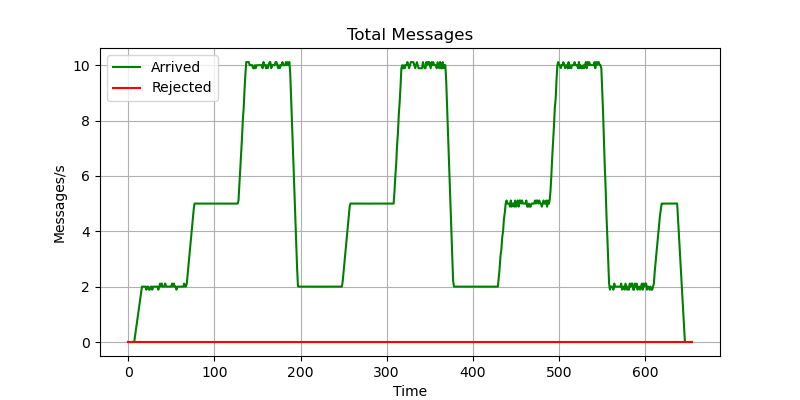
\includegraphics[width=0.85\linewidth]{images/Uniform_Fast/messages.png}
    \caption{Arrived and Rejected messages per second to the Queue.}
    \label{fig:uniform_fast_messages}
\end{figure}
\begin{figure}[H]
    \centering
    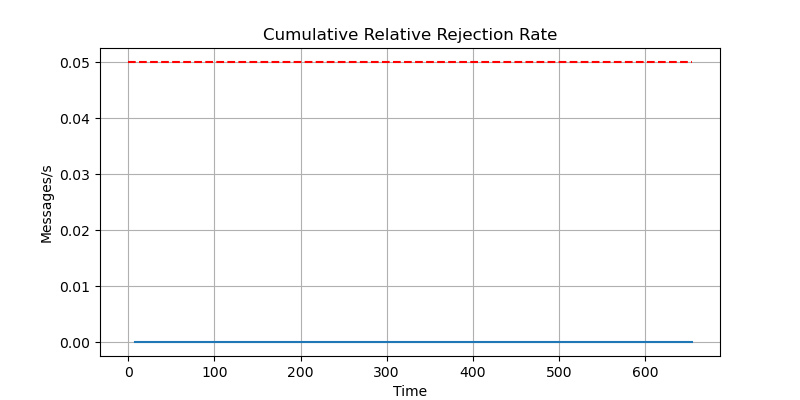
\includegraphics[width=0.85\linewidth]{images/Uniform_Fast/rejectiob_cumulative.png}
    \caption{Cumulative rejection rate.}
    \label{fig:uniform_fast_rejection}
\end{figure}
\begin{figure}[H]
    \centering
    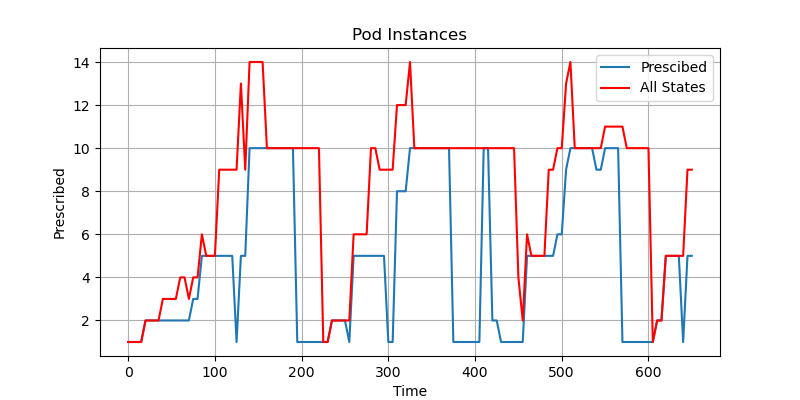
\includegraphics[width=0.85\textwidth]{images/Uniform_Fast/pods.png}
    \caption{In blue the number of pods prescribed by the scaler, the red one pods in all states.}
    \label{fig:uniform_fast_pods}
\end{figure}
\begin{figure}[H]
    \centering
    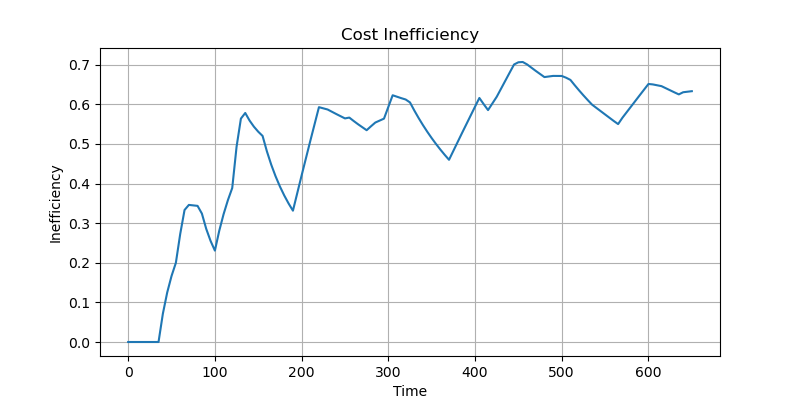
\includegraphics[width=0.85\linewidth]{images/Uniform_Fast/inefficiency_cumulative.png}
    \caption{At every time $t$, we calculate the inefficiency from starting time.}
    \label{fig:uniform_fast_inefficiency}
\end{figure}
\newpage
\subsection{Exponential}
\begin{figure}[H]
    \centering
    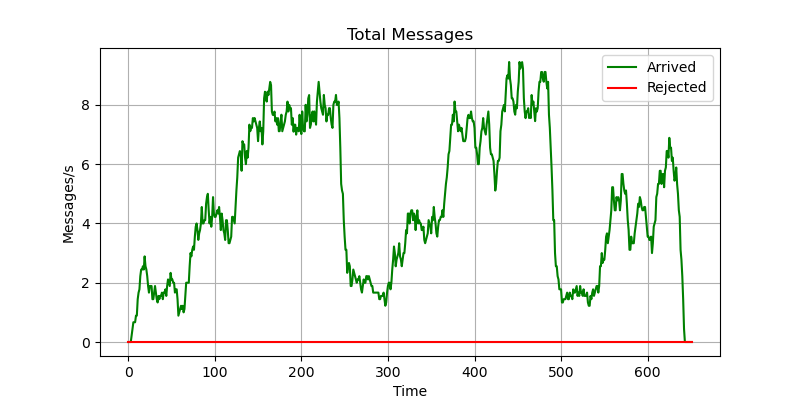
\includegraphics[width=0.85\linewidth]{images/Exponential/messages.png}
    \caption{Arrived and Rejected messages per second to the Queue.}
    \label{fig:exponential_messages}
\end{figure}

\begin{figure}[H]
    \centering
    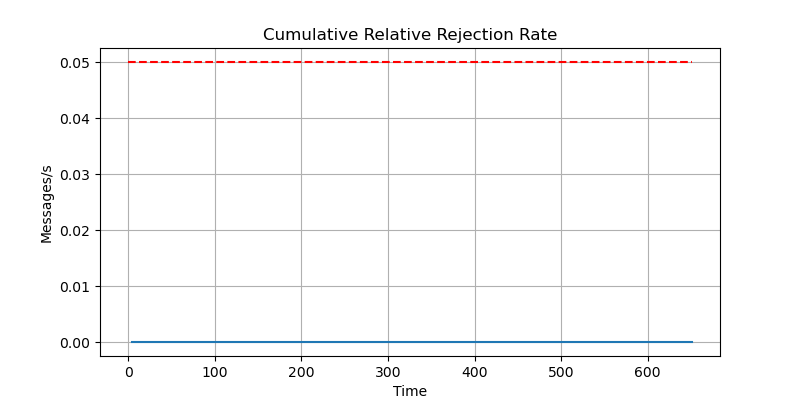
\includegraphics[width=0.85\linewidth]{images/Exponential/rejectiob_cumulative.png}
    \caption{Cumulative rejection rate.}
    \label{fig:exponential_rejection}
\end{figure}

\begin{figure}[H]
    \centering
    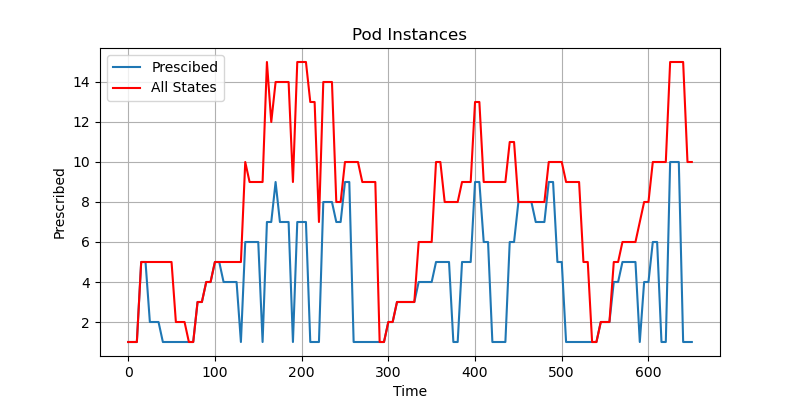
\includegraphics[width=0.85\textwidth]{images/Exponential/pods.png}
    \caption{In blue the number of pods prescribed by the scaler, the red one pods in all states.}
    \label{fig:exponential_pods}
\end{figure}
\begin{figure}[H]
\centering
    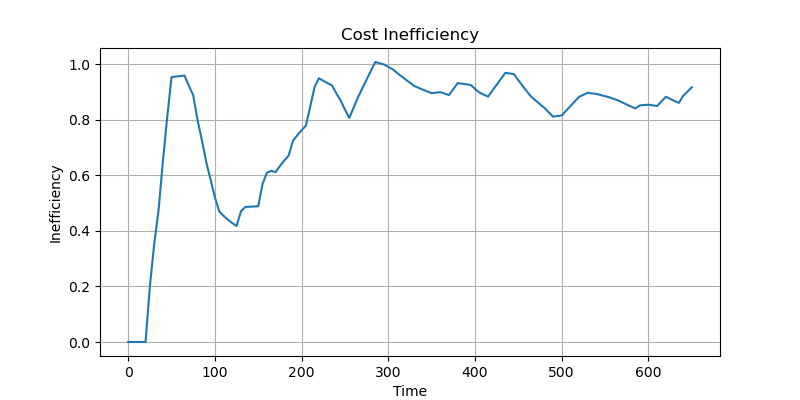
\includegraphics[width=0.85\linewidth]{images/Exponential/inefficiency_cumulative.png}
    \caption{At every time $t$, we calculate the inefficiency from starting time.}
    \label{fig:exponential_inefficiency}
\end{figure}